\documentclass[DM,lsstdraft,authoryear,toc]{lsstdoc}
% lsstdoc documentation: https://lsst-texmf.lsst.io/lsstdoc.html

% Package imports go here.
\usepackage{xspace}
\usepackage{hyperref}
\usepackage{graphicx}

% Local commands go here.
\newcommand{\opsim}{\texttt{OpSim}\xspace}
\newcommand{\socs}{\texttt{SOCS}\xspace}
\newcommand{\sched}{\texttt{Scheduler}\xspace}
\newcommand{\simsky}{\texttt{sims\_skybrightness}\xspace}
\newcommand{\magasq}{magnitude/arcsecond$^{2}$\xspace}

% To add a short-form title:
% \title[Short title]{Title}
\title{A New Baseline Operations Simulation}

% Optional subtitle
% \setDocSubtitle{A subtitle}

\author{%
Lynne Jones, 
Owen Boberg,
Tiago Ribeiro,
Kem Cook,
Andrew Heyer,
\v{Z}eljko Ivezi\'{c}
Colin Winslow
}

\setDocRef{baseline-opsim}

\date{\today}

% Optional: name of the document's curator
% \setDocCurator{The Curator of this Document}

\setDocAbstract{%
We present an update to the baseline simulated survey, created using \opsim v4. The last operations simulation baseline simulated survey was minion\_1016, produced in 2016. This simulated survey was produced using \opsim v3. The changes include updates to the sky brightness, significant changes in the underlying opsim scheduling software, and the addition of new scheduler parameters. 
}

% Change history defined here.
% Order: oldest first.
% Fields: VERSION, DATE, DESCRIPTION, OWNER NAME.
% See LPM-51 for version number policy.
\setDocChangeRecord{%
  \addtohist{1}{YYY-MM-DD}{Unreleased.}{Lynne Jones}
}

\begin{document}

% Create the title page.
% Table of contents is added automatically with the "toc" class option.
\maketitle

\section{Overview}

The new \opsim v4 codebase makes significant changes when compared with the previous \opsim v3 software. These include: 
\begin{itemize}
\item Separation of the telemetry and telescope control simulation software from the scheduler software. These two packages are now called \texttt{Simulated Observatory Control System} (\socs) and \texttt{Scheduler}. 
\item Implement communication between \socs and \sched via DDS, a publish/subscribe protocol that will be used to communicate between various telescope control systems, including the scheduler code.
\item Add a per-filter sky brightness calculation, using the \simsky package to calculate sky brightness values. This updates the sky brightness values to a model that includes a much higher fidelity twilight component and which has been validated against all-sky measurements from the LSST site. It also means that for each visit, the sky brightness limit is compared against the actual sky brightness estimate in the individual filter, instead of just against the $V$ band sky brightness as in \opsim v3.
\item Update the slew time cost function, to add further flexibility to prioritize short slews.
\item Add an additional cost to changing the filter, to reduce the number of filter changes and in particular, fast filter changes.
%\item Add the capability to restrict observations to a specified number of visits in a particular filter for a given field, per night. {\it E.g.}, limit visits for a given field to only 2 in $g$ band. This does not mean that no other visits to the same field will take place in the same night, but they would be in other filters which still have available groups. 
\item Add the capability to balance observations between different proposals (`time balancing'), as a function of progress toward the total number of requested observations. {\it E.g.}, space the 180 visits per field for the South Celestial Pole proposal over the entire survey, at the same pace as the 825 visits per field for the Wide Fast Deep proposal, so all proposals span the entire survey.
\item Add the capability to add a per-proposal `airmass bonus`, which adds a preference for low-airmass observations to the observation ranking algorithm.
\item Add the capability to add a per-proposal `Hour Angle bonus`, which adds a preference for low-hour angle observations to the observation ranking algorithm. 
\end{itemize}

Here we present a select list (see Table \ref{tab:runlist}) of simulated surveys created with \opsim v3 and v4, to illustrate the effects of these new features. First we compare minion\_1016 (the \opsim v3 baseline) with its original sky brightness and 5$\sigma$ limiting magnitudes to the same run, but with a newly calculated sky brightness value generated with the \simsky package and updated 5$\sigma$ limiting magnitudes, to generate an updated range of expected sky brightness and limiting magnitudes. Then we generated an \opsim v4 simulated survey without using the new features such as the time balancing or airmass or Hour Angle bonuses -- astro-lsst-01\_2020 -- to evaluate the general small changes between \opsim v3 and v4. We then generated a run adding time balancing to evaluate this effect, in colossus\_2432.  We compared a series of runs with varying airmass and hour angle bonuses to evaluate the effects of these bonuses, finding that a modest Hour Angle bonus worked the best for preserving survey uniformity while increasing the efficiency of the survey by obtaining observations in better conditions. We recommend adopting the new \opsim v4 simulated survey astro-lsst-01\_2022 as the new baseline run.

\begin{table}[htp]
\caption{Short list of simulated surveys illustrating \opsim changes.}
\begin{center}
\begin{tabular}{ l | l | l }
\opsim Run & Version & Summary \\
\hline
minion\_1016\_oldsky & \opsim v3 & Previous baseline, with old sky brightness values. \\
minion\_1016\_newsky &  & Previous baseline, reprocessed with new \simsky values.\\
astro-lsst-01\_2020 & \opsim v4  & All new features turned off (reproduce minion\_1016) \\
colossus\_2432 &  & Add time-balancing (TB).\\
colossus\_2328 &  & TB, Add restrict group visits (GV), and mild $HA$ bonus=0.05. \\
astro-lsst-01\_2016 &  & TB, GV, Add airmass bonus, $X$ bonus = 0.5 \\
astro-lsst-01\_2021 & & TB, GV, Add $HA$ bonus=0.5, $HA_{max}$=6 \\
astro-lsst-01\_2013 &  & TB, GV, Add $HA$ bonus=0.5, $HA_{max}$=3 \\
colossus\_2378 &  &  TB, GV, Add $HA$ bonus=0.8, $HA_{max}$=6 \\
astro-lsst-01\_2022 &   & TB, GV, Add $HA$ bonus=0.3, $HA_{max}$=3 \\
% colossus_2327 & & no time balancing, yes grouped visits
% colossus_2371 &  & no time balancing, no grouped visits
% colossus_2399 & & TB, GV, HA bonus 0.5 HAmax 6 
\end{tabular} 
\end{center}
\label{tab:runlist}
\end{table}

\section{Summary of skybrightness changes}

One of the major updates between \opsim v3 and v4 was the introduction of a higher fidelity sky brightness model, including a model for twilight. 

The \opsim v3 model was based on \citet{1991PASP..103.1033K} (K\&S), which provides a $V$ band sky brightness based on field airmass, lunar distance, and lunar phase. The \opsim v3 model added varying color terms appropriate for different lunar phases, along with a significant (but constant) bump in skybrightness to 17.0 \magasq to model twilight. The $y$ band skybrightness was additionally modeled as constant at 17.3 \magasq during the night to reflect a lower sensitivity to lunar brightness.  The big jump in sky brightness during twilight, combined with sky brightness limits set in the configuration files, in practice typically prevented filters other than $z$ and $y$ band being used during twilight\footnote{Sometimes observations were taken with \opsim v3 which violated the specified sky brightness limits. These were usually due to calculating the sky brightness values prior to twilight and caching the results through the transition to twilight.}.

\opsim v4 uses the \simsky package \citep{2016SPIE.9910E..1AY}, which is based on the ESO SkyCalc Sky Model Calculator  (v1.4) for non-twilight sky brightness calculations with an added empirical twilight sky model. The sky brightness calculated for each field depends on the field alt/az position, the lunar alt/az, the lunar phase, the sun alt/az, and the filter of the observation. It includes contributions from emission from the upper and lower atmosphere, scattered starlight, scattered moonlight, and zodiacal light, along with an additional component of scattered sunlight during twilight (sun altitude between -11 and -20 degrees). The transitions into and out of twilight are much smoother, and notably, the twilight sky can be darker than the specified sky brightness limits even in $u$ band near zenith. Thus in runs produced with \opsim v4.1, sometimes observations in $u$, $g$, $r$ or $i$ are taken during twilight due to a simple hard-limit on the sky brightness. It is possible to set these limits strictly enough to avoid this, however then some non-twilight observations at higher airmass, smaller distances to the moon, or at greater lunar phases, will also be ruled out, leaving significantly less flexibility in scheduling `normal' observations. In the future, the hard-limit will be replaced by a soft-constraint bonus, such as a preference for observations closer to the theoretical darkest sky brightness possible at a given time. 

%https://community.lsst.org/t/comparing-eso-sky-model-to-current-opsim-sky-values/489/2
%https://github.com/rhiannonlynne/notebooks/blob/master/skybright%20changes.ipynb

To evaluate the effect of changing the sky brightness model, we first reprocessed the previous baseline, minion\_1016, using \simsky. The overall changes in skybrightness range between from very slight (in $r$ band) to almost a magnitude decrease in skybrightness (in $z$ band). In general, the sky brightness gets fainter; $r$ band is the only filter where it gets brighter, and this is a very small change (see Table~\ref{tab:medskybright}). These changes are {\it after} including the observing conditions for each observation -- thus these results are averaged over a variety of lunar phases, airmass values, and field pointings. The effect the skybrightness reprocessing is consistent whether it is evaluated simply for all observations in a given bandpass or  for observations at a particular point in the sky in a given bandpass. We see roughly similar skybrightness values in \opsim v4 run astro-lsst-01\_2020, which was intended to reproduce minion\_1016 behavior, as it did not use any additional new features introduced by \opsim v4, even though v4 is now choosing observations based on the actual \simsky values in each bandpass (see Figure~\ref{fig:skybrightness}). 

\begin{table}[htp]
\caption{Median skybrightness over all observations in each filter, in minion\_1016, before and after reprocessing with \simsky.}
\begin{center}
\begin{tabular}{lrrr}
{} &  minion\_1016\_oldsky &  minion\_1016\_newsky &    Change \\
\hline
Median skyBrightness WFD u band       &           22.047386 &           22.706190 &  0.658804 \\
Median skyBrightness WFD g band       &           21.777833 &           22.071565 &  0.293732 \\
Median skyBrightness WFD r band       &           21.071279 &           21.027822 & -0.043457 \\
Median skyBrightness WFD i band       &           19.903494 &           20.055430 &  0.151936 \\
Median skyBrightness WFD z band       &           17.502343 &           18.646489 &  1.144146 \\
Median skyBrightness WFD y band       &           17.300000 &           17.774622 &  0.474622 \\
\hline
\end{tabular}
\end{center}
\label{tab:medskybright}
\end{table}


\begin{figure}[ht]
\centering
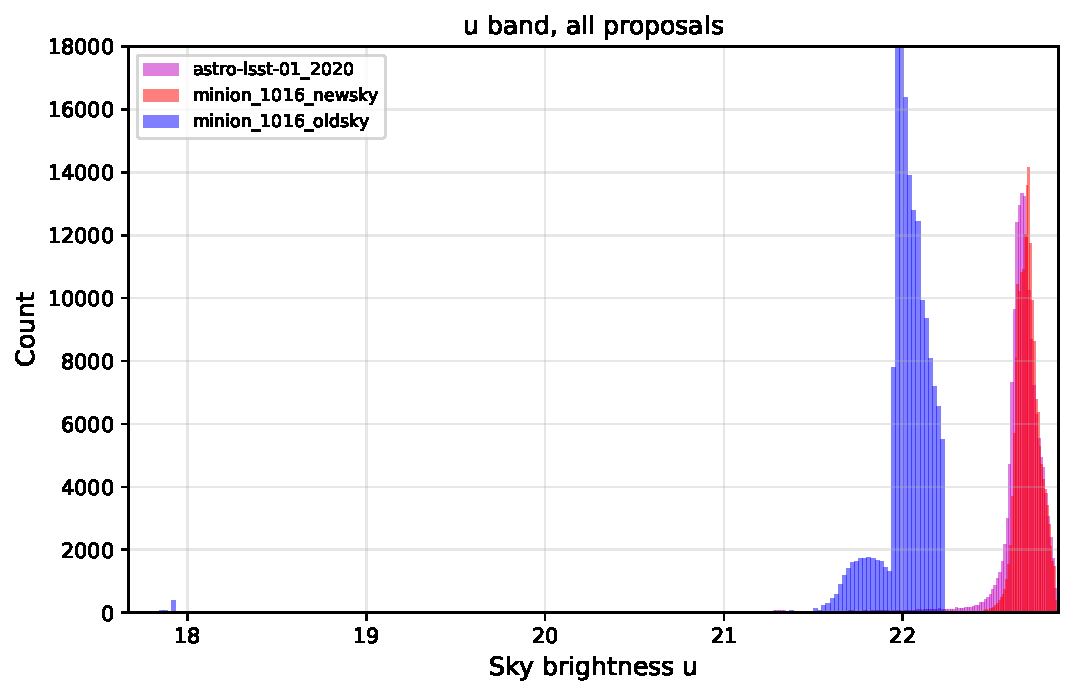
\includegraphics[width=0.3\textwidth]{figures/skybrightness_u_band_ONED_ComboBinnedData}
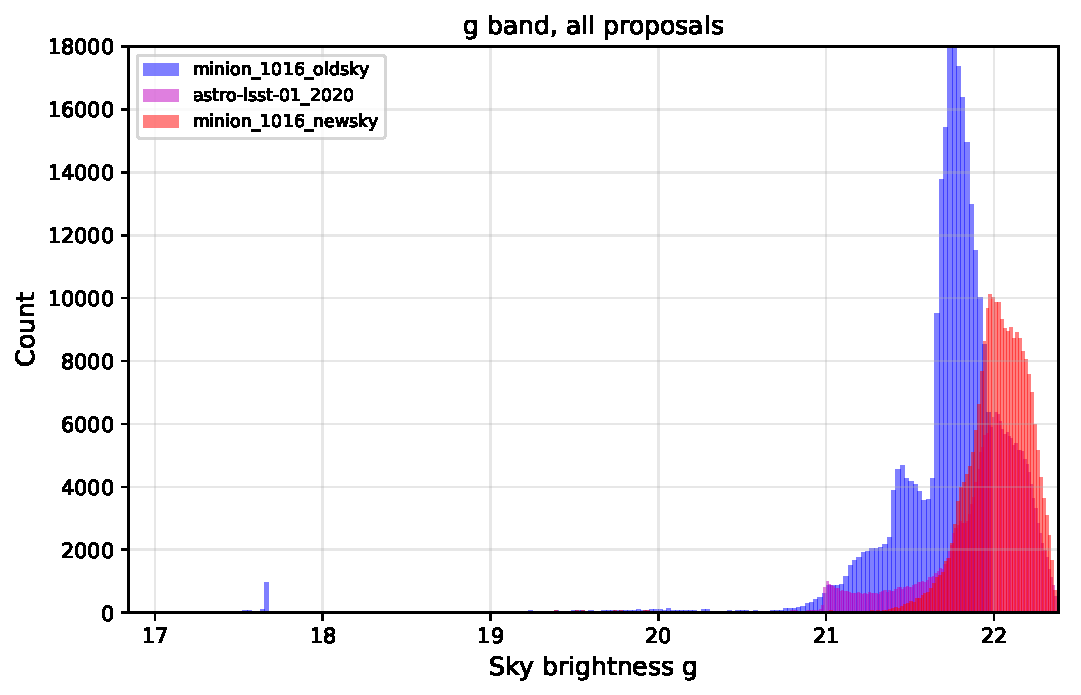
\includegraphics[width=0.3\textwidth]{figures/skybrightness_g_band_ONED_ComboBinnedData}
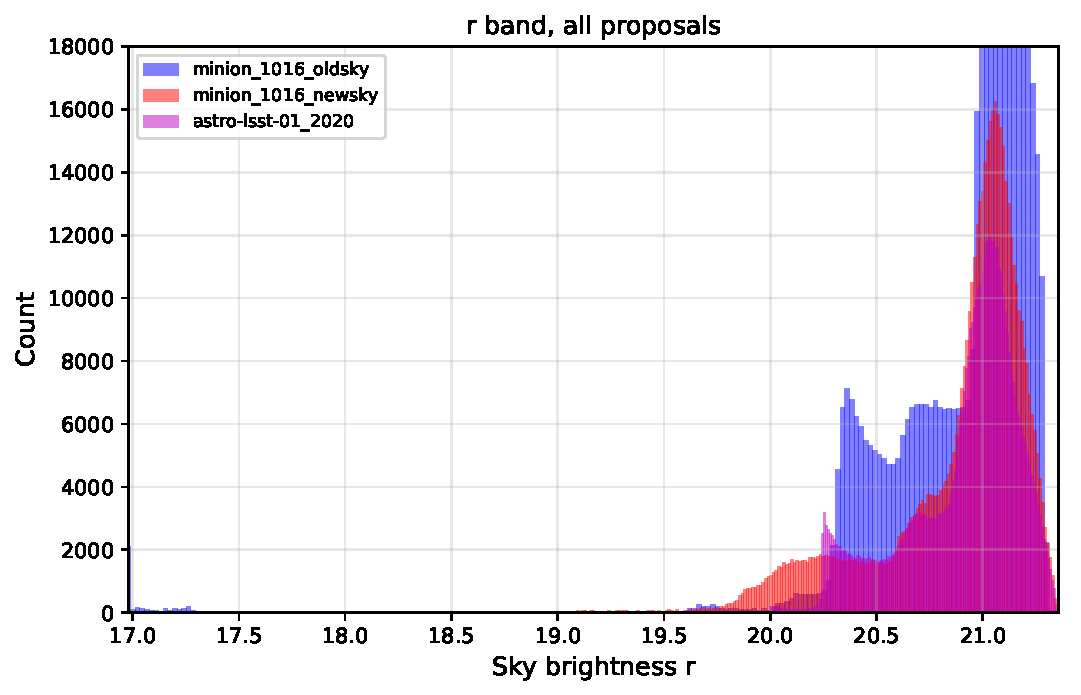
\includegraphics[width=0.3\textwidth]{figures/skybrightness_r_band_ONED_ComboBinnedData} \\
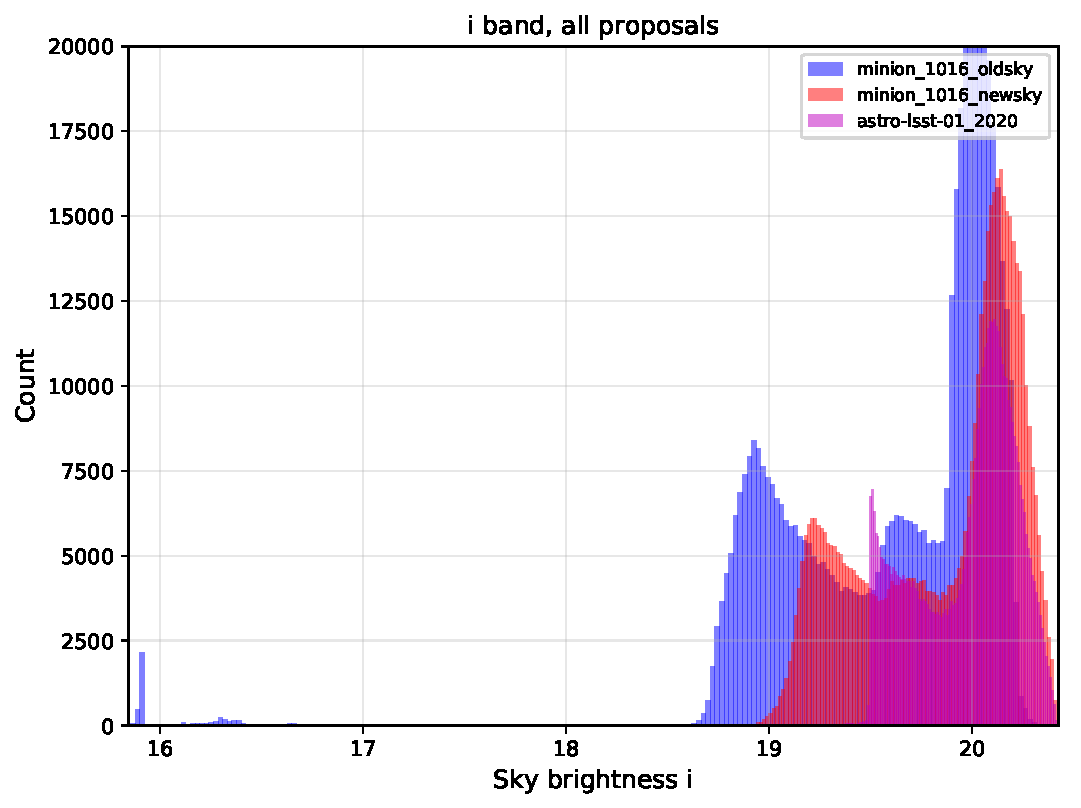
\includegraphics[width=0.3\textwidth]{figures/skybrightness_i_band_ONED_ComboBinnedData}
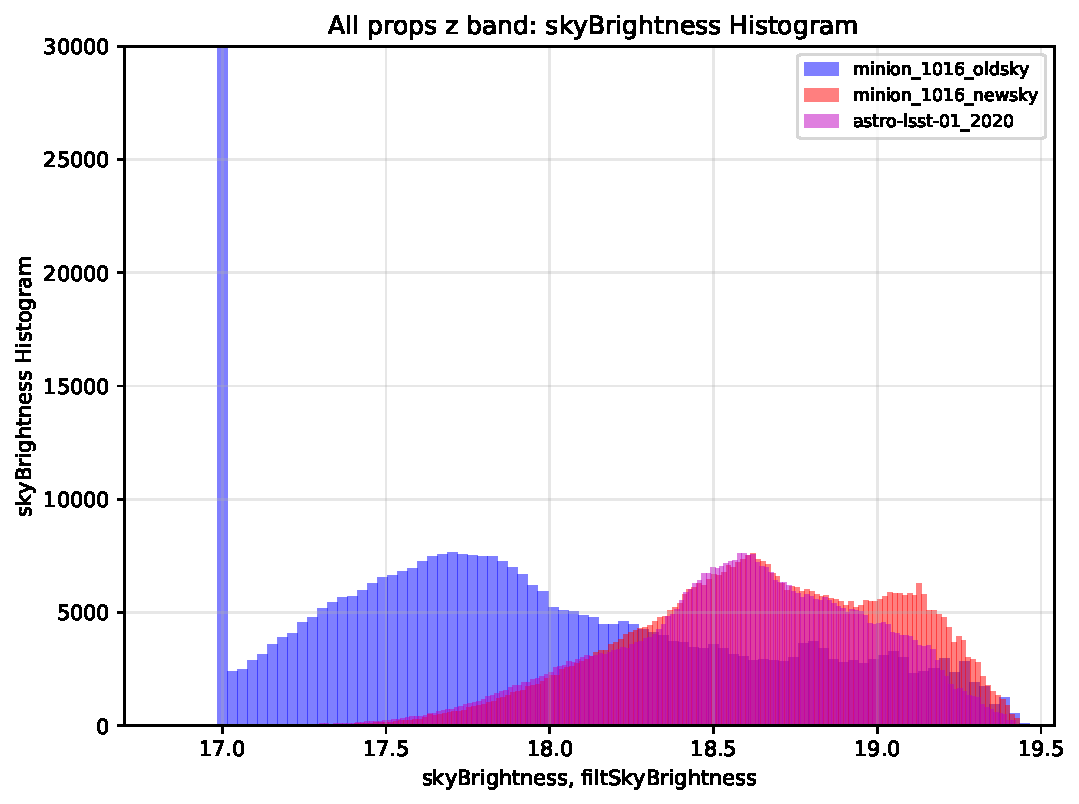
\includegraphics[width=0.3\textwidth]{figures/skybrightness_z_band_ONED_ComboBinnedData}
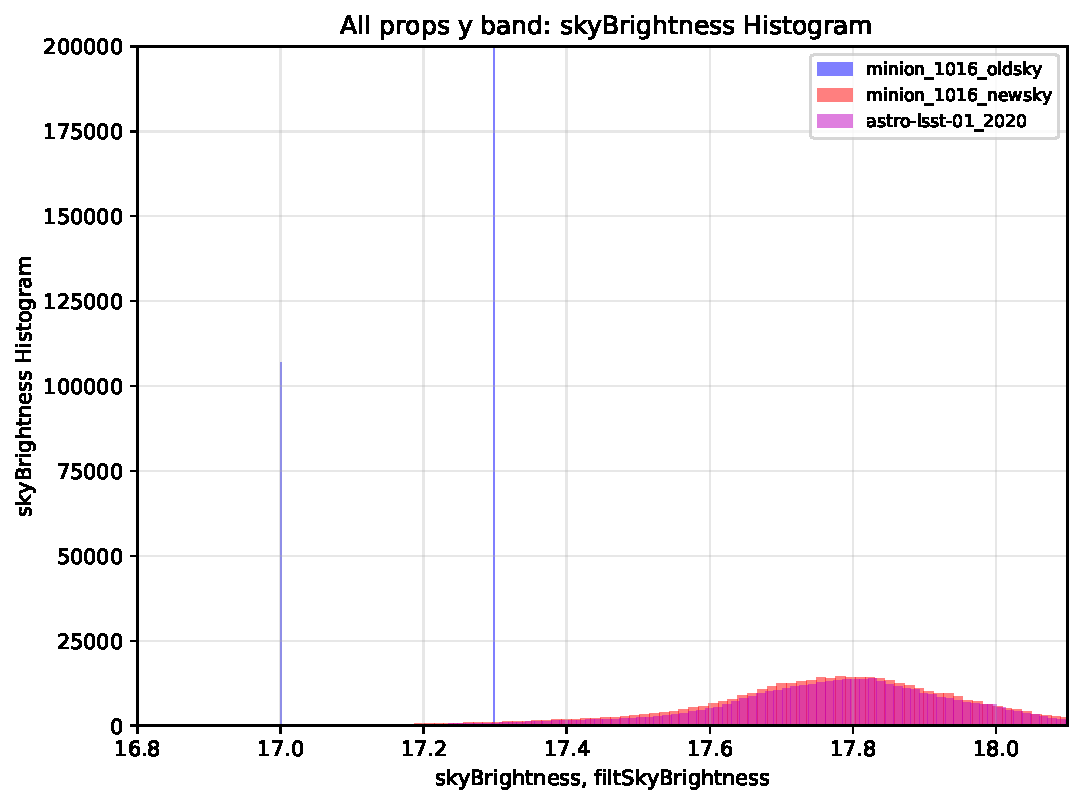
\includegraphics[width=0.3\textwidth]{figures/skybrightness_y_band_ONED_ComboBinnedData}
%\vskip -0.2in
\caption{Sky brightness histograms for minion\_1016 before (minion\_1016\_oldsky) and after (minion\_1016\_newsky) reprocessing with \simsky, and astro-lsst-01\_2020 skybrightness values. The values for astro-lsst-01\_2020 are very similar to the distribution seen in minion\_1016, even though \opsim v4 makes decisions for field pointings based on a knowledge of these skybrightness values in each filter at each pointing, information which was not available for \opsim v3. The changes in skybrightness, and resulting changes in 5$\sigma$ limiting magnitudes, we see due to reprocessing minion\_1016 are thus reasonable to expect in new \opsim v4 runs.
\label{fig:skybrightness}}
\end{figure}

The effect of these decreases in sky brightness are a resulting increase in the 5$\sigma$ limiting depths. There was, however, also an update in the expected throughput of the LSST system after the time of the original minion\_1016 limiting magnitude calculations, and this is also reflected in the change seen in the 5$\sigma$ depths. The throughput changes resulted in an overall decreased sensitivity, an effect which is strongest in the $u$ and $g$ bands. See Table~\ref{tab:m5depth} for the median 5$\sigma$ limiting magnitudes per visit in the WFD observations. 

\begin{table}[ht]
\caption{Individual image 5$\sigma$ limiting magnitudes for minion\_1016 before and after reprocessing with \simsky, and astro-lsst-01\_2020. The changes in limiting magnitude correspond to 0.5 times the change in skybrightness, appropriate for the change in SNR, but there were additional changes in the expected throughput of the telescope included in the reprocessing that result in the final m5 changes being slightly smaller than expected.}
\begin{center}
\begin{tabular}{lrrr}
{} &  minion\_1016\_oldsky &  minion\_1016\_newsky &  astro-lsst-01\_2020 \\
\hline
Median m5 WFD u band &           23.137883 &           23.111817 &           23.079406 \\
Median m5 WFD g band &           24.472729 &           24.545191 &           24.474827 \\
Median m5 WFD r band &           24.153684 &           24.085377 &           24.072373 \\
Median m5 WFD i band &           23.392901 &           23.470681 &           23.542878 \\
Median m5 WFD z band &           22.223935 &           22.759990 &           22.720512 \\
Median m5 WFD y band &           21.571697 &           21.800913 &           21.819558 \\
\hline
\end{tabular}
\end{center}
\label{tab:m5depth}
\end{table}

\section{Effect of changing the slew time and filter change cost functions}

The slew time cost function changed slightly between \opsim v3 and v4, substituting an equation that is parametrized by $t_{ref}$, $c_{ref}$, and $t_{max}$, where $t_{ref}$ is intended to be the `reference' slew, $c_{ref}$ is the standard cost of that reference slew, and $t_{max}$ represents the time of a very long slew. The slew time cost function increases rapidly over a range of short slews, and then increases slowly when approaching $t_{max}$.  The cost associated with a range of slew times, with the standard parameters is illustrated in Figure~\ref{fig:slewcost}.  The resulting distribution of slew times in the \opsim v3 baseline, minion\_1016, and the \opsim v4 run with the major new features turned off, astro-lsst-01\_2020, are very similar for short slews, while once into the long slew regime, v4 allows longer slews more often.

\begin{figure}[ht]
\centering
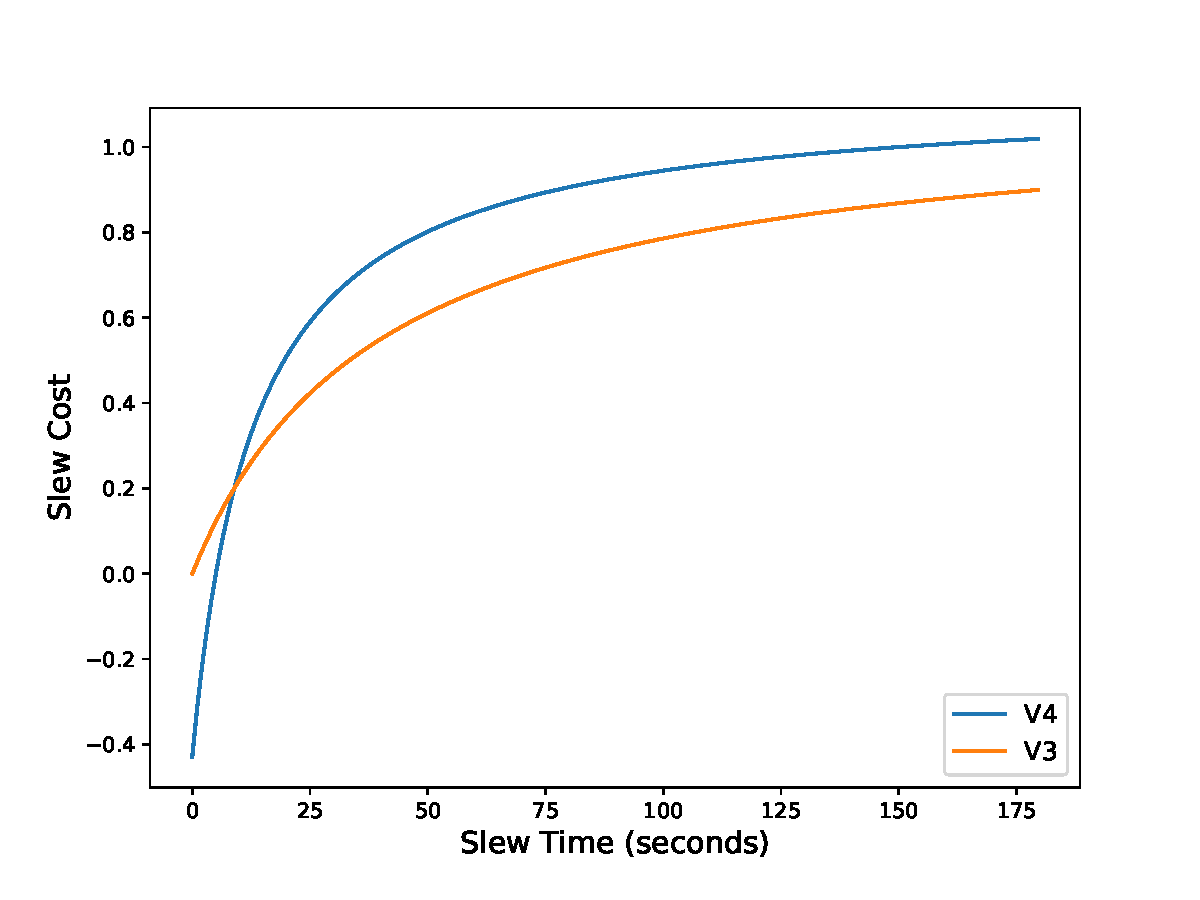
\includegraphics[width=0.37\textwidth]{figures/slewcost}
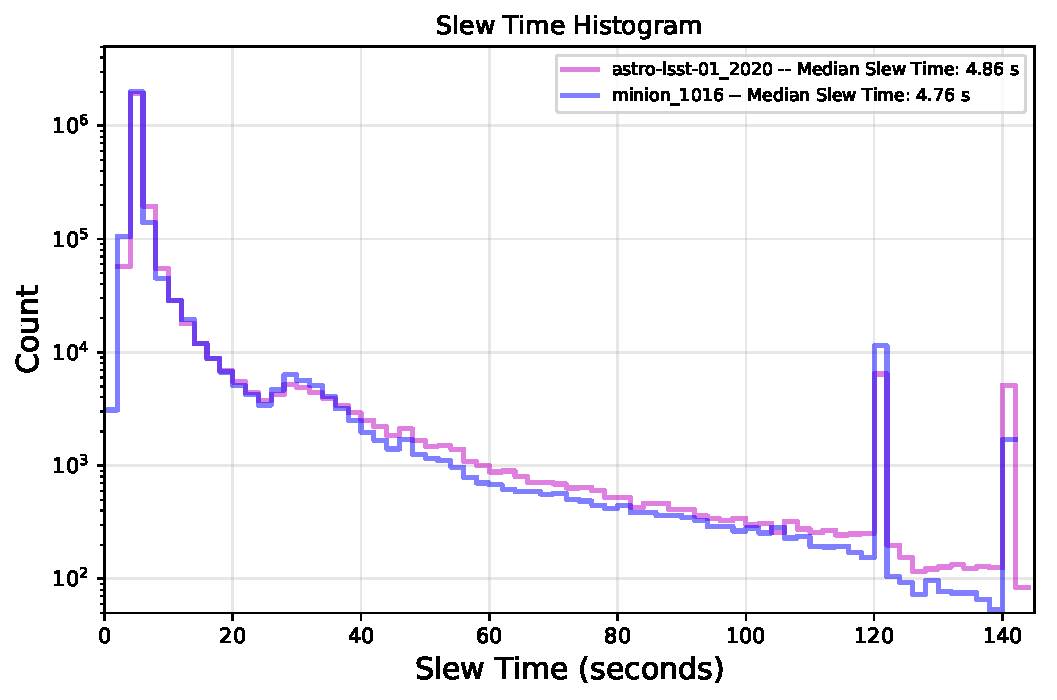
\includegraphics[width=0.4\textwidth]{figures/slewtimes}
\caption{Left: Slew time cost associated with a given slew time, using the default values for $t_{ref}$ (5s), $c_{ref}$ (0.3) and $t_{max}$ (150s). The slew time required is determined by the model of the telescope movement. The cost associated with that slew time is used in the ranking algorithm for choosing the next target in the scheduler. Right: The distribution of slew times in minion\_1016 and astro-lsst-01\_2020 (an \opsim v4 simulation run without new v4 features). 
\label{fig:slewcost}}
\end{figure}

The filter change cost calculation was also changed between \opsim v3 and v4, in order to reduce the number of filter changes, particularly on a rapid timescale. The result is that astro-lsst-01\_2020 has 11213 total filter changes, compared to 14194 for minion\_1016; over 20\% fewer filter changes in the new survey. The overall number of filter changes in each of the new simulated surveys is similar; between 10,000 -- 12,000 filter changes over the lifetime of the survey. 

\section{The addition of time-balancing}

A significant problem in minion\_1016 was that different proposals within the simulated survey completed their observations at different rates. The proposals which requested fewer total visits than the WFD would reach their requested number of visits before the nominal survey baseline of 10 years, instead of spacing the visits out over time appropriately. \opsim v4 adds the capability to rank targets by the overall progress of each proposal towards its total goal number of visits. This means that the rate of acquiring visits for each proposal remains more uniform over the survey lifetime. 

\begin{figure}[ht]
\centering
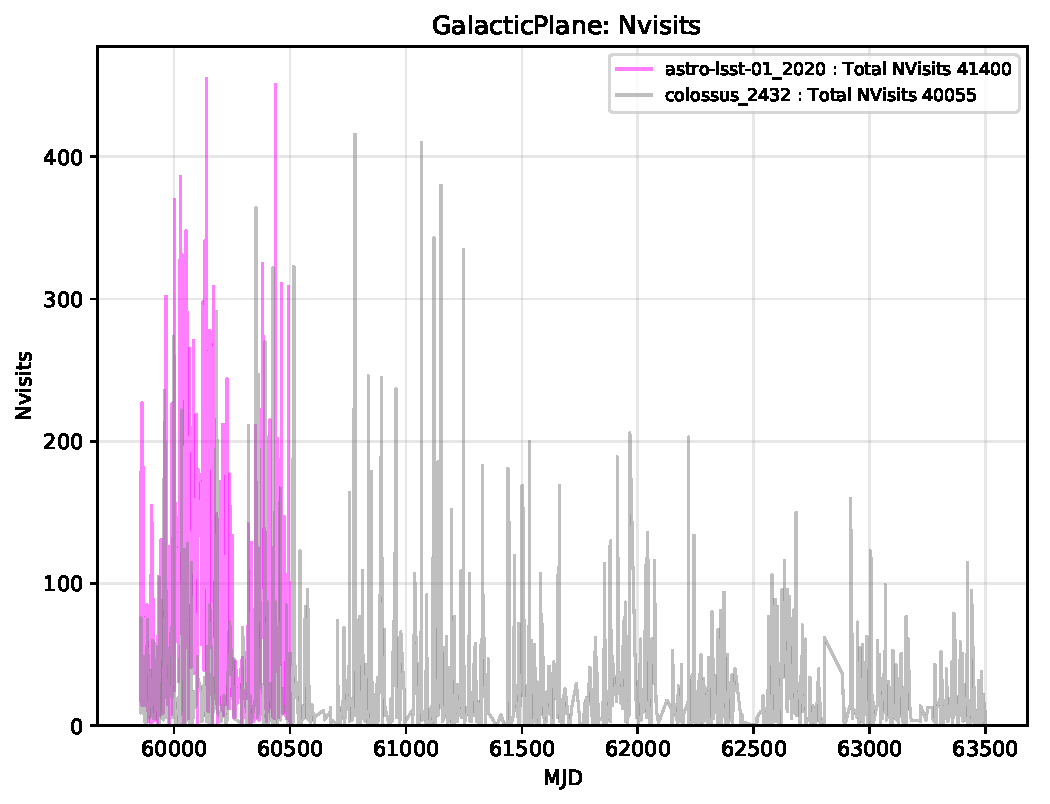
\includegraphics[width=0.3\textwidth]{figures/timebalancing_gp}
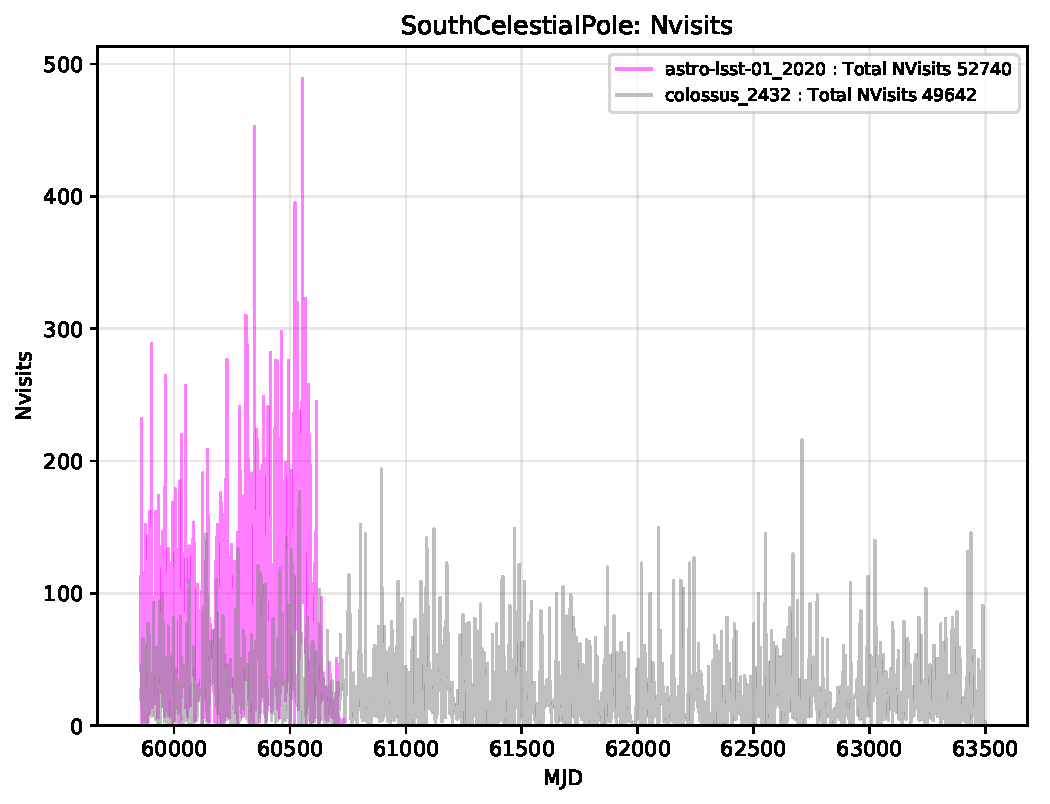
\includegraphics[width=0.3\textwidth]{figures/timebalancing_scp}
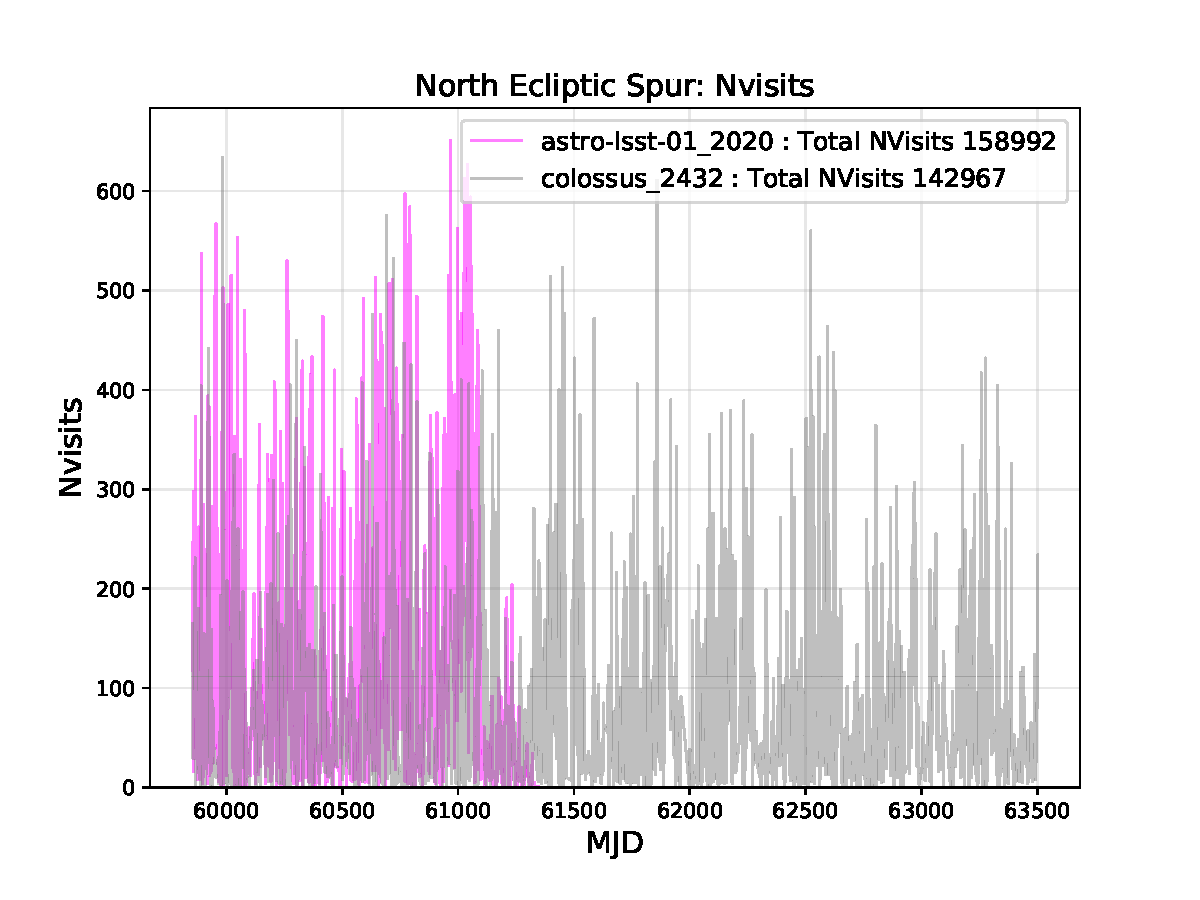
\includegraphics[width=0.3\textwidth]{figures/timebalancing_nes}
\caption{The galactic plane proposal and south celestial pole proposal only request 30 visits per field, per filter. The north ecliptic spur proposal requests about 1/3 of the visits of the full WFD per field. In minion\_1016 and astro-lsst-01\_2020 (an \opsim v4 run without time balancing), these proposals obtained all of their observations only a few years into the survey. With time balancing turned on, the rate of acquiring observations is slower and visits are obtained throughout the simulated lifetime of LSST.
\label{fig:timebalancing}}
\end{figure}


\section{Choosing the bonus values} 

\opsim v4 provides the capability to choose observations that prefer low airmass (via the 'airmass bonus') or low hour angle angle (via the 'hour angle bonus'). We investigated ..
(2 year blocks of X bonus vs 2 year blocks of HA bonus)


\section{New baseline survey recommendation}

The SRD places requirements on the amount of sky which receives a given minimum number of visits (table 22) and the number of visits over a given minimum area (table 23). Together these specifications are that 18,000 square degrees should receive at least 825 visits (together known as the `fO' metrics). The performance of each of these simulated surveys regarding this important metric is shown in Figure~\ref{fig:srd}. The top panel in the figure illustrates the minimum number of visits an 18,000 sq degree area receives (Nvisits/825 line) and the amount of area covered which receives at least 825 visits (Area/18k sq deg line).  The bottom panel illustrates the changes in the number of visits in each simulated survey, together with the `effective time' of each survey. Effective time is defined as the equivalent amount of on-sky time a survey would require to reach the same limiting magnitudes as the total coadded depths, assuming all observations were actually taken in a fiducial set of observing conditions. If the actual observations are obtained in bad conditions (high airmass, bright sky backgrounds), the effective time is smaller; if observations are taken with good conditions, the effective time is larger.

In the v3 baseline, minion\_1016, the SRD fO metric values were relatively high, as the overall number of visits was larger. With \opsim v4, the airmass or hour angle bonuses add preferences for observations in better conditions (closer to the meridian) but which result in longer slew times. This reduces the overall number of visits but increases the effective time of the survey. The fO metrics fail when these bonuses are set to particularly strong values, primarily because the observations are spread more unevenly over the sky. Observing close to the meridian in some regions of $RA$ is difficult due to the arrangement of the Deep Drilling fields and the North Ecliptic Spur. With a fewer number of overall visits, this pushes some areas down below the benchmark (825 visits) value, causing these fO metric values to fall below the required thresholds. 

\begin{figure}[ht]
\centering
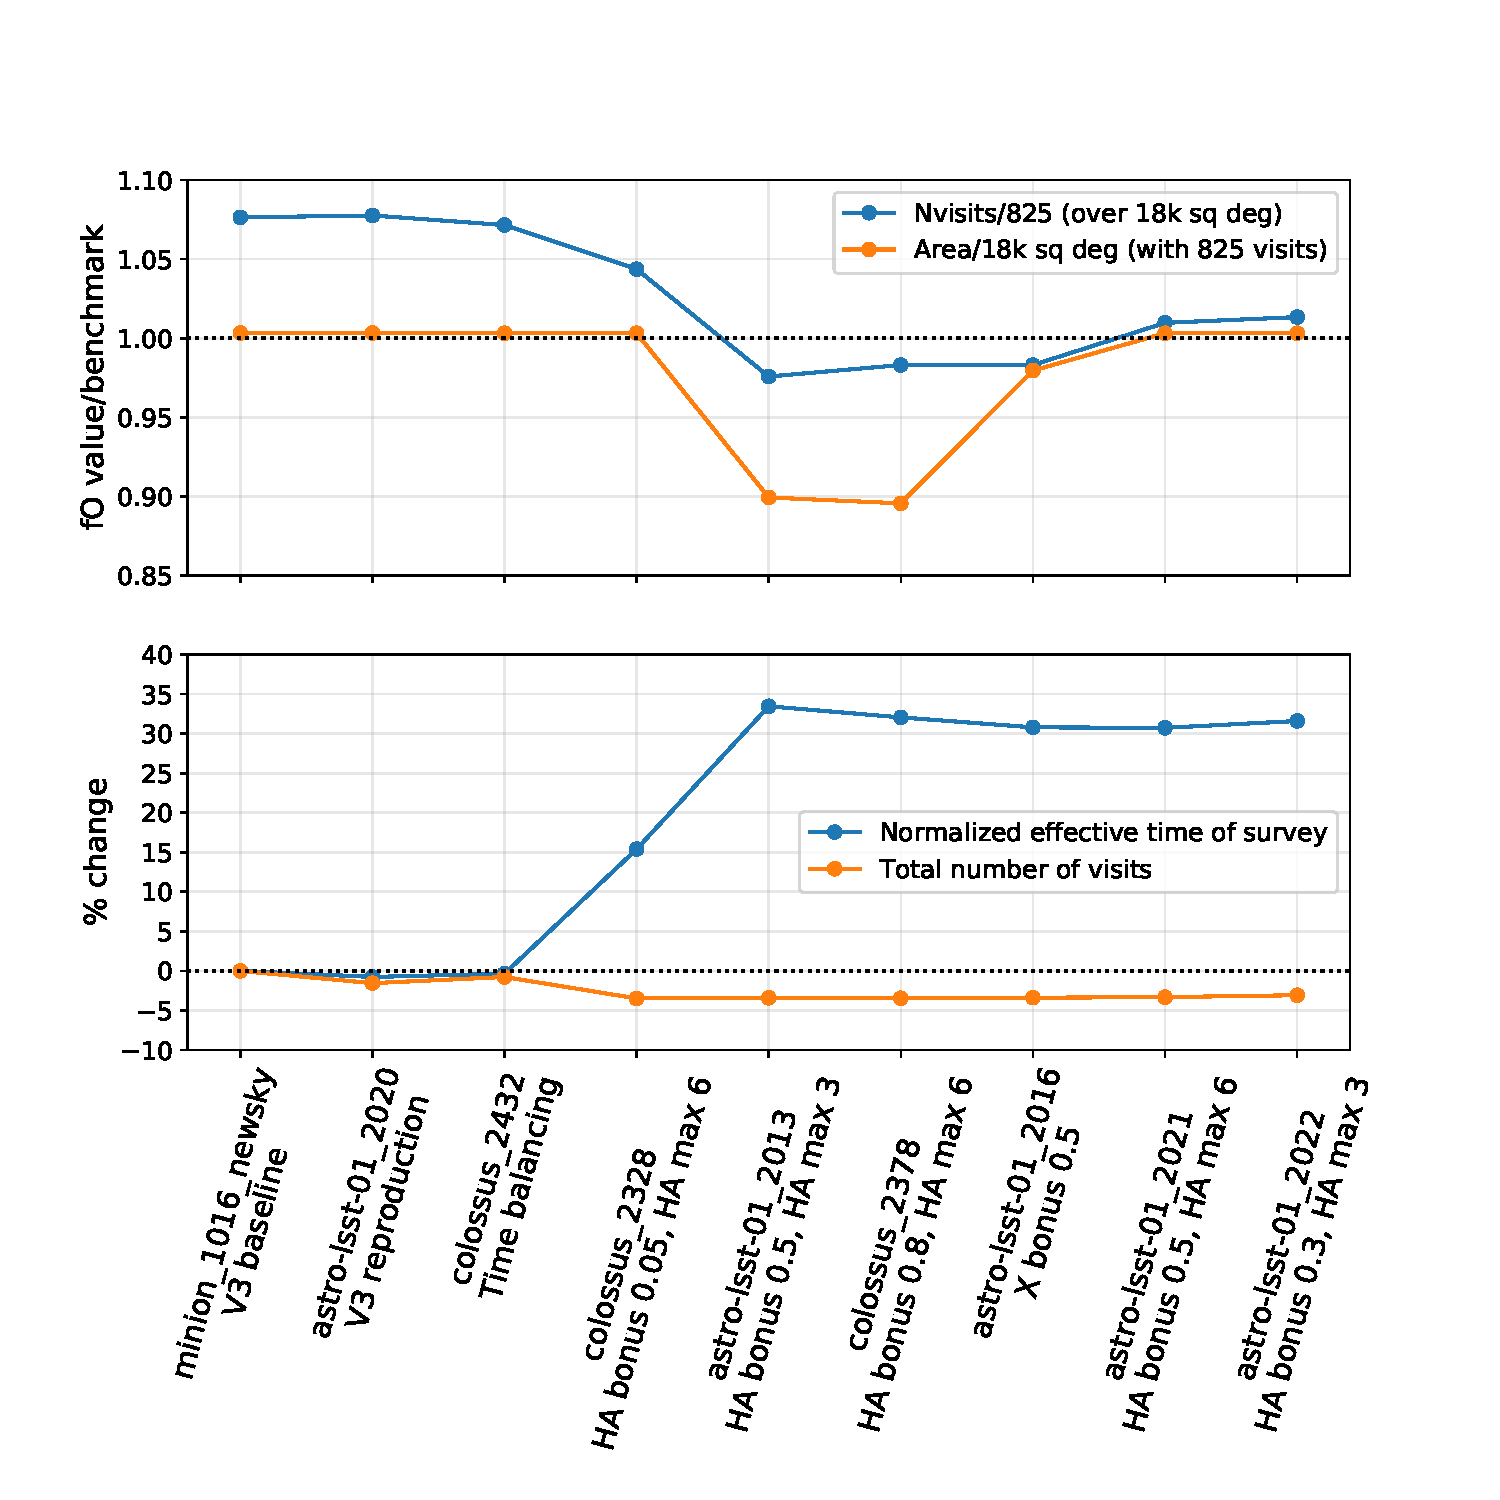
\includegraphics[width=0.9\textwidth]{figures/srd}
%\vskip -0.2in
\caption{The top panel in figure illustrates the minimum number of visits an 18,000 sq degree area receives (Nvisits/825 line) and the amount of area covered which receives at least 825 visits (Area/18k sq deg line).  The bottom panel illustrates the changes in the number of visits in each simulated survey, together with the `effective time' of each survey. Effective time is defined as the equivalent amount of on-sky time a survey would require to reach the same limiting magnitudes as the total coadded depths, assuming all observations were actually taken in a fiducial set of observing conditions. If the actual observations are obtained in bad conditions (high airmass, bright sky backgrounds), the effective time is smaller; if observations are taken with good conditions, the effective time is larger.
\label{fig:srd}}
\end{figure}

\begin{figure}[ht]
\centering
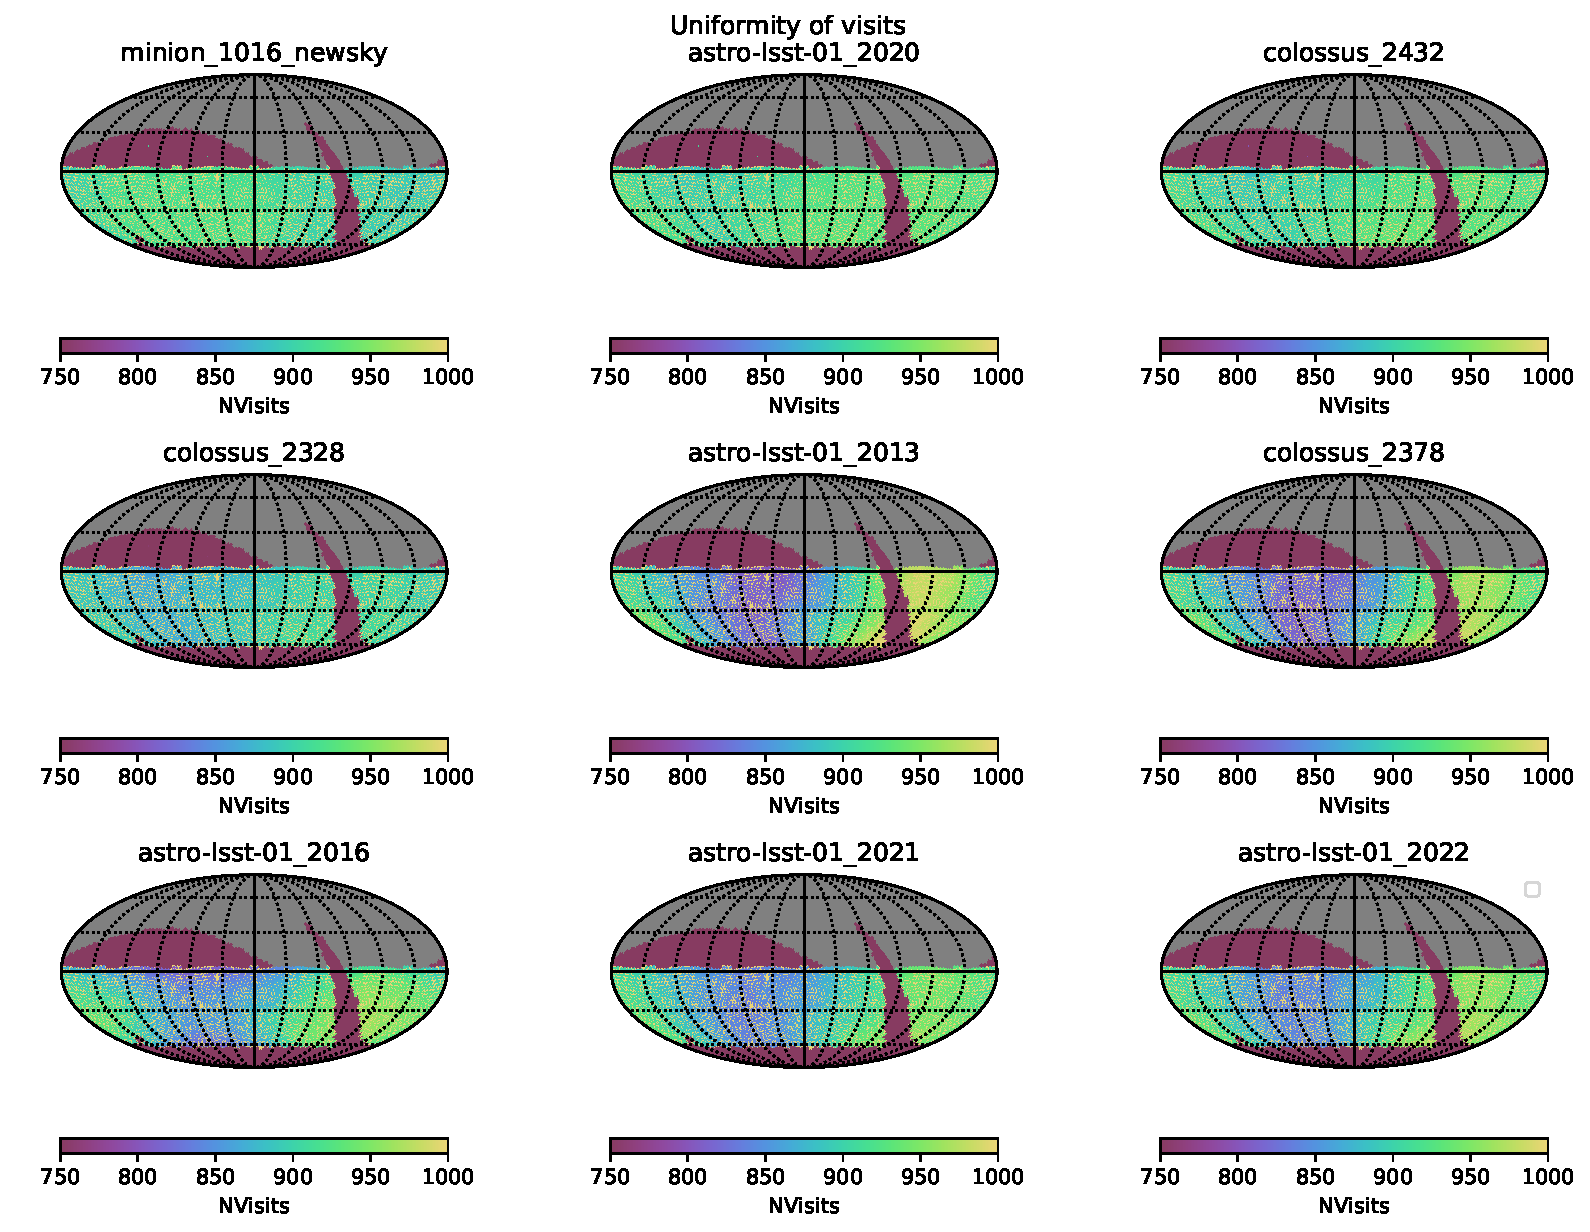
\includegraphics[width=0.9\textwidth]{figures/uniformity_of_visits}
%\vskip -0.2in
\caption{Stronger preferences for observing near the meridian (strong $HA$ bonus coupled with small $HA_{max}$ values) or zenith (strong $X$ bonus) result in more nonuniformity in visits across the WFD. Figure~\ref{fig:uniformity_dd} illustrates that this is correlated to the location of Deep Drilling fields and the location of the North Ecliptic Spur.
\label{fig:uniformity_all}}
\end{figure}

\begin{figure}[ht]
\centering
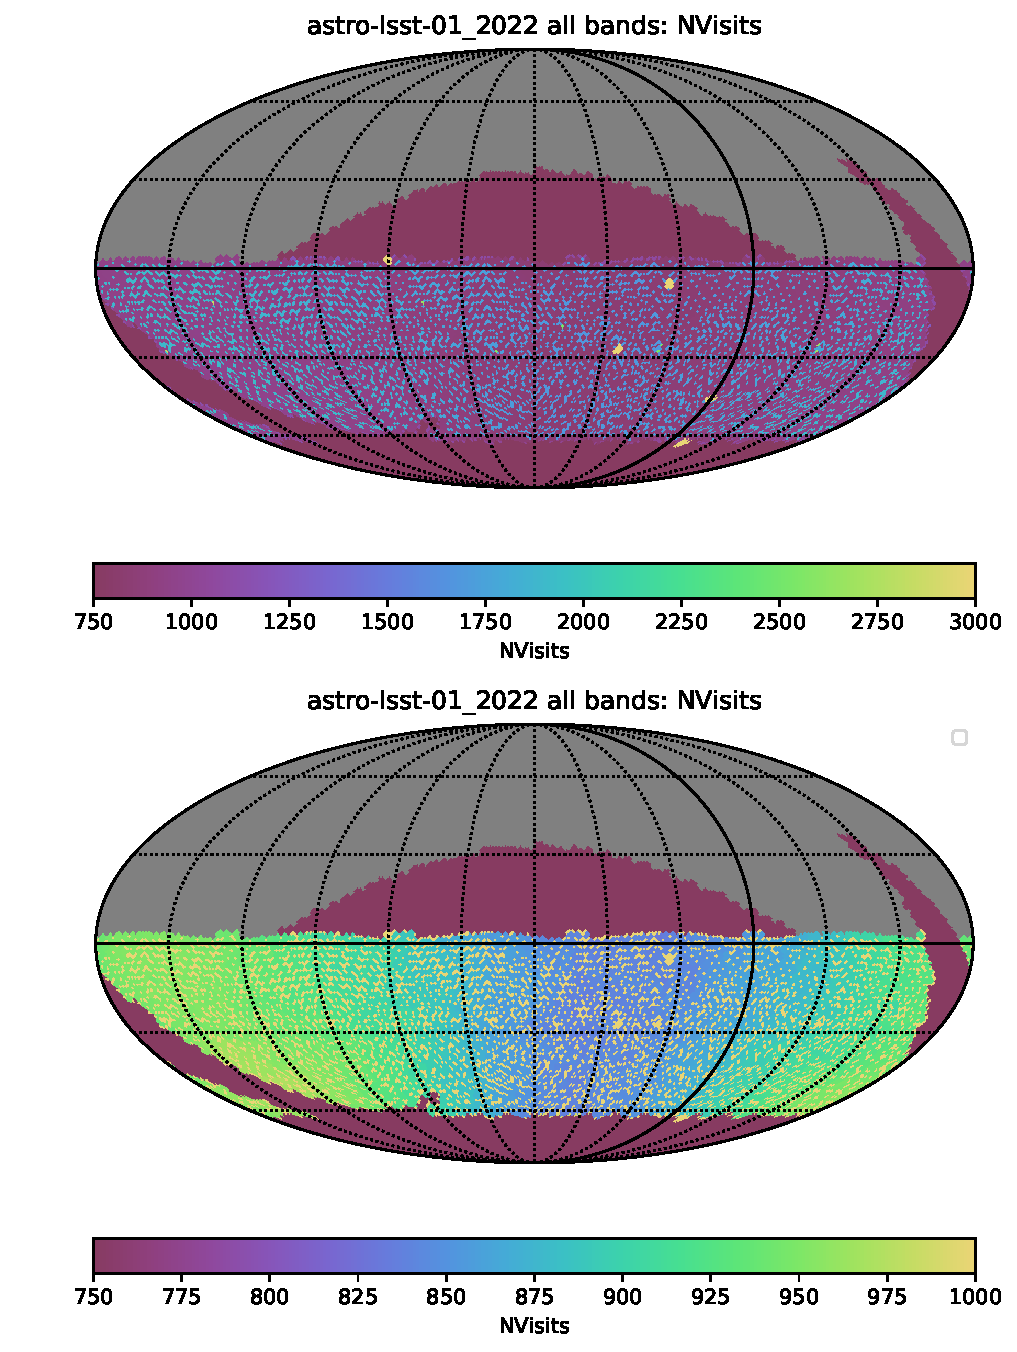
\includegraphics[width=0.6\textwidth]{figures/uniformity_dd}
%\vskip -0.2in
\caption{The nonuniformity in visits, when adding stronger preferences for observing near the meridian, is correlated with the locations of the Deep Drilling fields, four of which are clumped within 30 degrees in $RA$, as well as an increased width of the North Ecliptic Spur. Improved methods to make the distribution of visits across all ranges of $RA$ more uniform will need to be investigated in future simulated surveys. 
\label{fig:uniformity_dd}}
\end{figure}


\begin{figure}[ht]
\centering
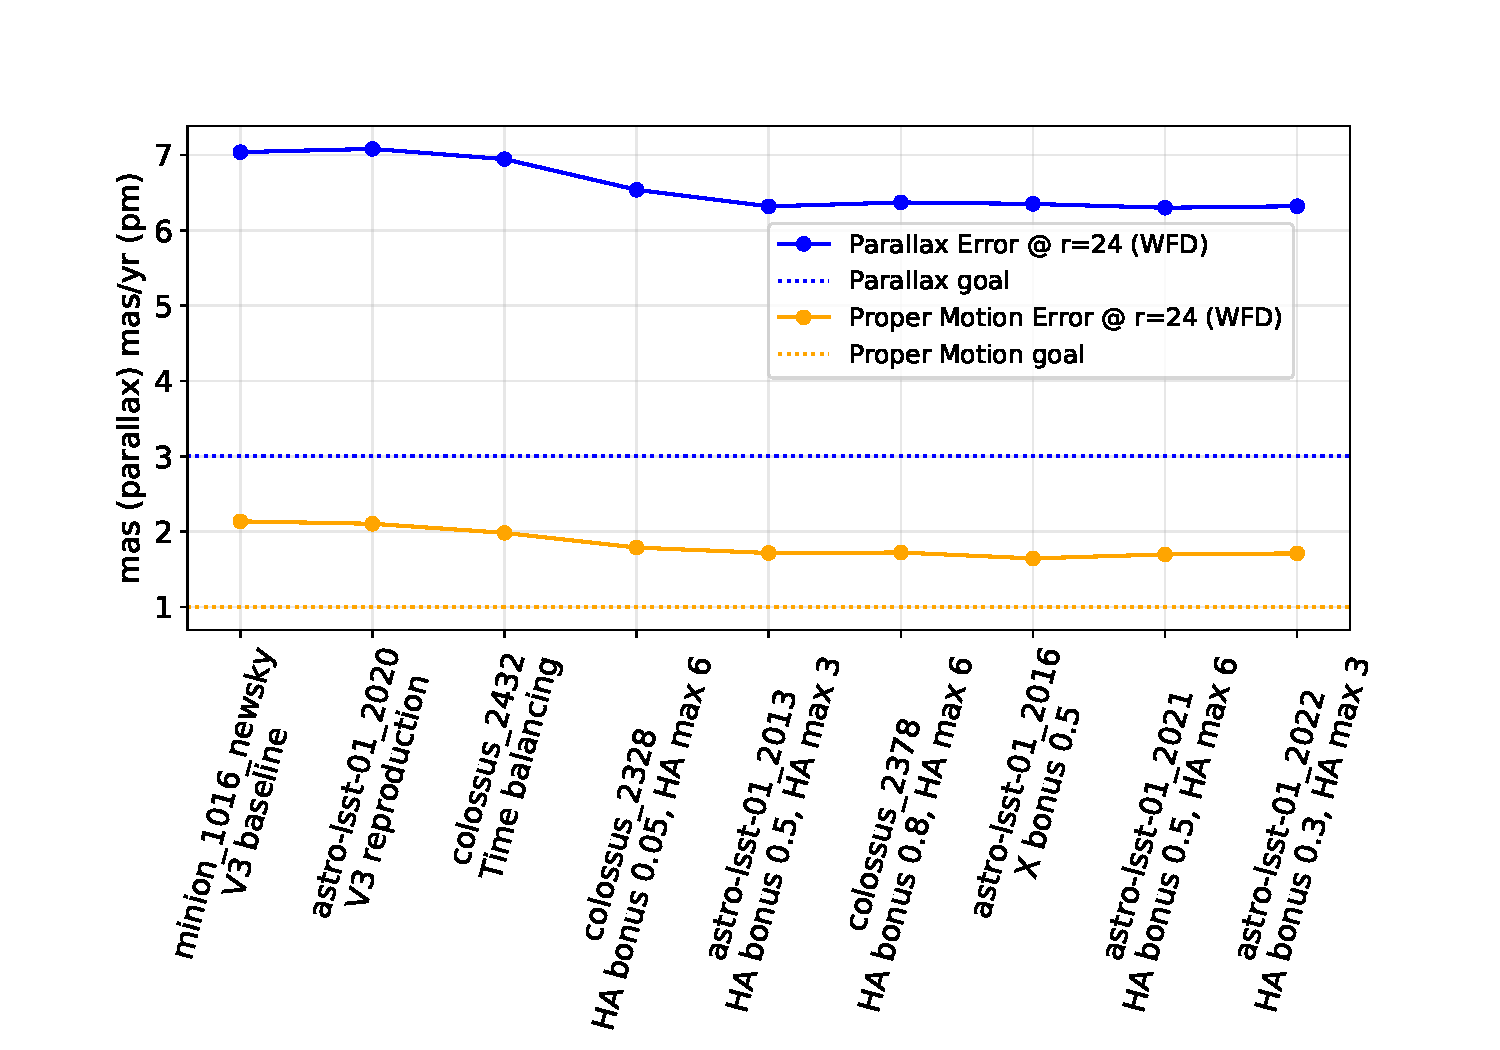
\includegraphics[width=0.9\textwidth]{figures/astrometry}
%\vskip -0.2in
\caption{
\label{fig:astrometry}}
\end{figure}




srd values pass

other big changes from minion\_1016

\section{Reproducibility of new baseline survey and its evaluation}

config files
results of evaluation
how they were produced
where they can be found online

% Include all the relevant bib files.
% https://lsst-texmf.lsst.io/lsstdoc.html#bibliographies
\bibliography{lsst,lsst-dm,refs_ads,refs,books}

\end{document}
